\documentclass[11pt]{article}
\usepackage[toc,page]{appendix}
\usepackage{amsmath, amssymb}
\usepackage[utf8]{inputenc}
\usepackage[T1]{fontenc}
\usepackage[style=apa,backend=biber]{biblatex}
%\usepackage{biblatex}
\addbibresource{references.bib}
\usepackage{graphicx}
\usepackage{tikz}
\usetikzlibrary{automata,positioning,shapes.geometric, arrows.meta, fit, backgrounds, calc, chains}
\graphicspath{./images/Easy_Pictures/SMR_MULT_Repackaging}%\usepackage{kpfonts}
\usepackage{float}
\usepackage[margin=1in]{geometry}
\usepackage{cancel}
\usepackage{epsfig}
\usepackage{tikz-3dplot}
\usepackage{darkmode}
\usepackage{dirtytalk}
\usepackage{longtable,booktabs,array}
\usepackage{calc} % for calculating minipage widths
\usepackage[utf8]{inputenc}
\usepackage[T1]{fontenc}
\usepackage{xcolor}
\usepackage{listings}


\usepackage{etoolbox}
\usepackage{hyperref}
\hypersetup{
 colorlinks=true,
 linkcolor=blue,
 filecolor=magenta, 
 urlcolor=cyan,
 pdftitle={Hermeneutic Calculator},
 citecolor=blue,
 }


\urlstyle{same}

\lstdefinestyle{htmlStyle}{
 language=HTML,
 basicstyle=\ttfamily\small,
 keywordstyle=\color{blue}\bfseries,
 commentstyle=\color{gray}\itshape,
 stringstyle=\color{red},
 breaklines=true,
 frame=single,
 numbers=left,
 numberstyle=\tiny\color{gray},
 columns=fullflexible,
}
\lstdefinelanguage{HTML}{
 keywords={<!DOCTYPE, html, head, title, body, h1, h2, h3, p, div, span, a, img, ul, li, table, tr, td, th, style, link, script},
 sensitive=true,
 comment=[l]{//},
 morecomment=[s]{/*}{*/},
 morestring=[b]',
 morestring=[b]"
}
\lstset{style=htmlstyle, language=html}
% Updated to explicitly pass the language option
%\lstinputlisting[style=htmlstyle, language=html]{./html/example.html}
%\usepackage{tocloft}

% Optional: define some custom colors
\definecolor{sliceRed}{RGB}{225,224,91} % matching "varyellow" from your code
\definecolor{linkYellow}{RGB}{255,215,0} % a golden yellow
\tdplotsetmaincoords{70}{110}

\title{Subtraction Strategies: Sliding to Make Bases}
\author{Compiled by: Theodore M. Savich}


\begin{document}
\maketitle
\subsection*{Transcript}
 Strategy descriptions and examples adapted from \textcite{HackenbergCourseNotes}. This is not based on a CGI video. I fake a student example. 

\begin{itemize}
\item Teacher: John had 73 pieces of halloween candy. He gave 47 pieces to his friend. How many pieces of candy does John have left?
\item Student: I can pretend I gave away 50 pieces and also pretend I had three more than I did. So that's like 76-50, which is 26. 
\end{itemize}

\noindent \textbf{Notation Representing Rita's Solution:}
\begin{align*}
    73 - 47 &= \Box\\
    73+3 &= 76\\
    47+3 &= 50\\
    73 - 47 &= 76 - 50\\
    &= 26
\end{align*}

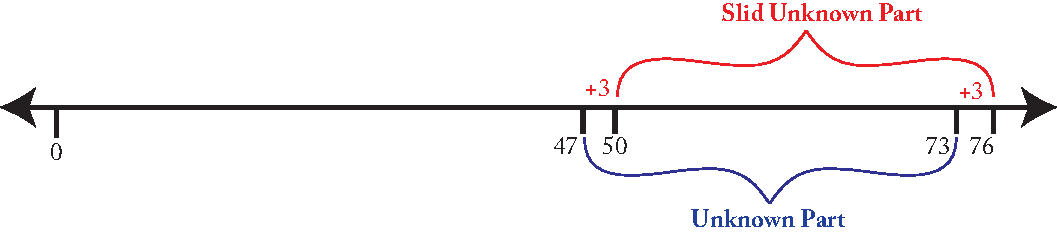
\includegraphics[width=.8\textwidth]{images/Easy_Pictures/SAR_SUB_Sliding/PDF/SAR_SUB_Sliding.pdf}

\noindent In the sliding strategy, you adjust both the number you’re subtracting from (the whole) and the number being subtracted (the part) by the same amount. The goal is to shift the subtrahend into a `friendly' number (usually a multiple of a base). By doing this, the difference between the adjusted values remains identical to the original difference, simplifying the subtraction process.


\subsubsection*{Description of Strategy}
\begin{itemize}
    \item \textbf{Objective:} Adjust both the minuend (known whole) and subtrahend (known part) by the same amount to make the subtraction easier, keeping the difference the same.
\end{itemize}

\subsubsection*{Corrected Automaton (Register Machine Model)}

We define a Register Machine that models the Sliding strategy, including the iterative subroutine to find the adjustment K.

**M = (Q, V, \delta, q_0, F)**

\begin{itemize}
    \item \textbf{States (Q):} {$q_{start}, q_{init\_K}, q_{loop\_K}, q_{adjust}, q_{subtract}, q_{accept}$}
    \item \textbf{Registers (V):} M, S, K (Adjustment), M\_adj, S\_adj, Result.
    \item \textbf{Internal Registers:} TempCounter, TargetBase.
\end{itemize}

**Transition Function (\delta):**

\begin{longtable}{|l|l|l|l|l|}
\hline
\textbf{Current State} & \textbf{Condition} & \textbf{Next State} & \textbf{Action} & \textbf{Interpretation} \\
\hline
\endhead
$q_{start}$ & (Input M, S) & $q_{init\_K}$ & - & Start. Target S for adjustment. \\
\hline
$q_{init\_K}$ & - & $q_{loop\_K}$ & K=0; Temp=S; TargetBase=NextBase(S) & Initialize "Count Up To Base" on S. \\
\hline
$q_{loop\_K}$ & **Temp < TargetBase** & $q_{loop\_K}$ & K+=1; Temp+=1 & Iteratively count up to find K. \\
\hline
$q_{loop\_K}$ & **Temp == TargetBase** & $q_{adjust}$ & - & K found. \\
\hline
$q_{adjust}$ & - & $q_{subtract}$ & S\_adj = S+K; M\_adj = M+K & Apply the slide K to both M and S. \\
\hline
$q_{subtract}$ & - & $q_{accept}$ & Result = M\_adj - S\_adj & Perform the simplified subtraction. \\
\hline
\end{longtable}

\subsubsection*{Automaton Diagram for Sliding to Make Bases}

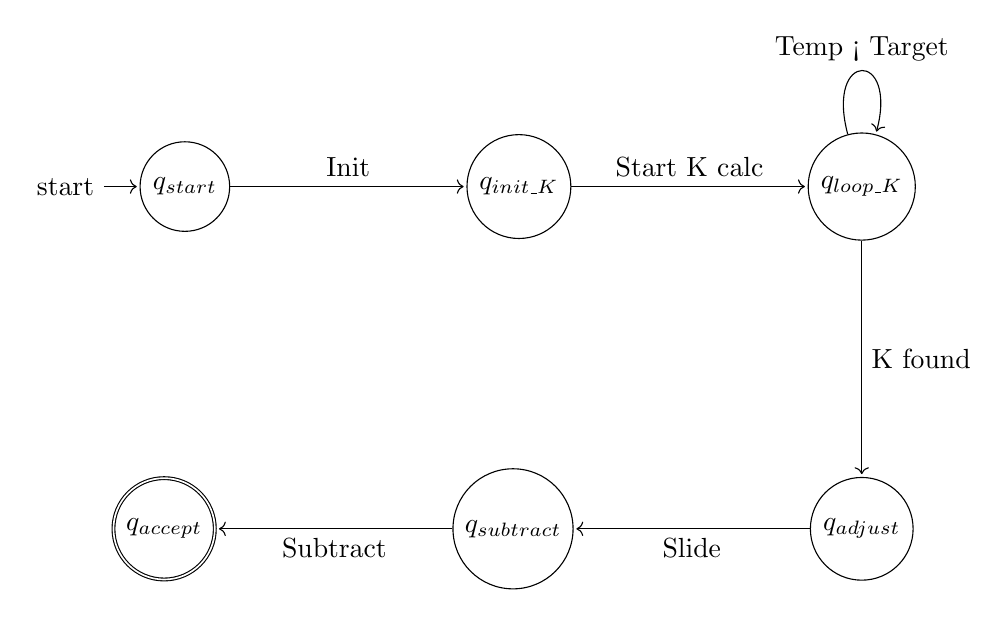
\begin{tikzpicture}[
    shorten >=1pt,
    auto,
    node distance=3cm,
    every state/.style={minimum size=1cm, align=center}
]
    % States
    \node[state, initial] (start) {$q_{start}$};
    \node[state, right=of start] (init_k) {$q_{init\_K}$};
    \node[state, right=of init_k] (loop_k) {$q_{loop\_K}$};
    \node[state, below=of loop_k] (adjust) {$q_{adjust}$};
    \node[state, left=of adjust] (subtract) {$q_{subtract}$};
    \node[state, accepting, left=of subtract] (accept) {$q_{accept}$};

    % Transitions
    \path[->]
        (start) edge node {Init} (init_k)
        (init_k) edge node {Start K calc} (loop_k)
        (loop_k) edge[loop above] node {Temp < Target} (loop_k)
        (loop_k) edge node {K found} (adjust)
        (adjust) edge node {Slide} (subtract)
        (subtract) edge node {Subtract} (accept);
\end{tikzpicture}

\subsubsection*{Python Implementation and Test}

\begin{lstlisting}[language=Python]
import pandas as pd
import math

class SlidingAutomaton:
    """
    A Register Machine model simulating the 'Sliding' (Constant Difference) strategy.
    Models the cognitive process including the iterative steps to calculate the adjustment K.
    """
    strategy_name = "Sliding to Make Bases (Constant Difference)"

    def __init__(self, M, S, Base=10):
        self.M = M
        self.S = S
        self.Base = Base
        self.history = []
        self.state = 'q_start'
        self.Result = 0

        # Main Registers
        self.K = 0
        self.M_adj = 0
        self.S_adj = 0

        # Internal registers for iteration
        self.TargetBase = 0
        self.TempCounter = 0

        if S > M:
            self.state = 'q_error'
            self._record_history(f"Error: Subtrahend ({S}) > Minuend ({M}).")

    def _record_history(self, interpretation, highlight=False):
        self.history.append({
            'State': self.state, 'Interpretation': interpretation,
            'K': self.K, 'M_adj': self.M_adj, 'S_adj': self.S_adj,
            'Highlight': highlight
        })

    def transition(self, next_state):
        self.state = next_state

    def run(self):
        while self.state not in ['q_accept', 'q_error']:
            executor = getattr(self, f"execute_{self.state}", self.execute_error)
            executor()
        return self.Result

    def execute_error(self):
        if self.state != 'q_error':
            self._record_history(f"Error: Entered unknown state {self.state}")
            self.transition('q_error')

    # --- State Execution Methods ---

    def execute_q_start(self):
        self._record_history(f"Inputs: M={self.M}, S={self.S}. Target S for adjustment.", highlight=True)
        self.transition('q_init_K')

    # Subroutine: Calculate K (Count Up To Base)
    def execute_q_init_K(self):
        """Initialize the 'Count Up To Base' subroutine on S."""
        self.K = 0
        self.TempCounter = self.S

        # Determine the target base (e.g., 47 -> 50)
        if self.S > 0 and self.S % self.Base != 0:
             # Calculate the next highest multiple of the base
             self.TargetBase = ((self.S // self.Base) + 1) * self.Base
        else:
             self.TargetBase = self.S # Already at a base or zero

        self._record_history(f"Initializing K calculation: Counting from {self.S} to {self.TargetBase}.")
        self.transition('q_loop_K')

    def execute_q_loop_K(self):
        """Iteratively count up to the base."""
        if self.TempCounter < self.TargetBase:
            # Primitive counting operation
            self.TempCounter += 1
            self.K += 1
            self._record_history(f"Counting Up: {self.TempCounter}, K={self.K}")
        else:
            self._record_history(f"K needed to reach base is {self.K}.", highlight=True)
            self.transition('q_adjust')

    def execute_q_adjust(self):
        """Apply K to both M and S (The Slide)."""
        self.S_adj = self.S + self.K # Should equal TargetBase
        self.M_adj = self.M + self.K
        self._record_history(f"Sliding both by +{self.K}. New problem: {self.M_adj} - {self.S_adj}.", highlight=True)
        self.transition('q_subtract')

    def execute_q_subtract(self):
        """Perform the simplified subtraction."""
        # This step is cognitively simple because S_adj is a base multiple.
        self.Result = self.M_adj - self.S_adj
        self._record_history(f"Perform Subtraction: {self.M_adj} - {self.S_adj} = {self.Result}.", highlight=True)
        self.transition('q_accept')

    def execute_q_accept(self):
         # Final state logic (if any additional recording is needed)
         pass

    def display_history(self, summarized=True):
        print(f"\n--- {self.strategy_name} History ({self.M} - {self.S}) ---")
        df = pd.DataFrame(self.history)
        display_cols = ['State', 'Interpretation', 'K', 'M_adj', 'S_adj']

        if summarized:
             print("Summary Trace:")
             summary_df = df[df['Highlight'] == True]
             if not summary_df.empty:
                print(summary_df[display_cols].to_markdown(index=False))
        else:
            print("Full Iterative Trace:")
            print(df[display_cols].to_markdown(index=False))

# Test Case: Example from PDF (73 - 47)
M_test = 73
S_test = 47
sliding_auto = SlidingAutomaton(M=M_test, S=S_test)
sliding_auto.run()
sliding_auto.display_history(summarized=False)
\end{lstlisting}

\subsubsection*{Execution Trace (73 - 47):}
\begin{verbatim}
--- Sliding to Make Bases (Constant Difference) History (73 - 47) ---
Full Iterative Trace:
| State      | Interpretation                                                 |   K |   M_adj |   S_adj |
|:-----------|:---------------------------------------------------------------|----:|--------:|--------:|
| q_start    | Inputs: M=73, S=47. Target S for adjustment.                   |   0 |       0 |       0 |
| q_init_K   | Initializing K calculation: Counting from 47 to 50.            |   0 |       0 |       0 |
| q_loop_K   | Counting Up: 48, K=1                                           |   1 |       0 |       0 |
| q_loop_K   | Counting Up: 49, K=2                                           |   2 |       0 |       0 |
| q_loop_K   | Counting Up: 50, K=3                                           |   3 |       0 |       0 |
| q_loop_K   | K needed to reach base is 3.                                   |   3 |       0 |       0 |
| q_adjust   | Sliding both by +3. New problem: 76 - 50.                      |   3 |      76 |      50 |
| q_subtract | Perform Subtraction: 76 - 50 = 26.                             |   3 |      76 |      50 |
\end{verbatim}

\printbibliography
\end{document}